\section{Documentation for system engineers}
\subsection{Compilation and download}
The program comes with a \texttt{Makefile} that can be used to compile the program. To this end, the right command to use is \texttt{make timer}. It will generate some files in the current directory (\texttt{.}) and in \texttt{./Objects/}. In order to download the program into the naked computer, the user should follow the following steps (supposing the router is correctly configured):
\begin{itemize}
	\item Run \texttt{tftp 192.168.97.60} in the same directory as \texttt{timer.c}. The \texttt{tftp} environment will start;
	\item \texttt{binary}, to send the program as binary;
	\item \texttt{trace}, to see what happens;
	\item \texttt{verbose}, to see more information;
	\item \texttt{put timer.hex}.
\end{itemize}
Please notice that the last command has to be run only when the board is ready to receive the program. This happens during the three seconds after its reboot.

\subsection{System clock frequency measurement}
The clock frequency of the board that is being used (Olimex PIC-MAXI-WEB) is set at boot time by the tftp server. To know exactly at what frequency the board is running, a test routine has been performed with an ad-hoc software (\texttt{clkfreq.c}).

To take the measurement another time reference is needed; the basic idea is to count how many execution clock ticks happen in a certain period and obtain the frequency from the inverse relationship.

In addition to the main clock, a second - low-frequency - oscillator (32.768 kHz) is present inside the Olimex board; using the full 16-bit register it is possible to count up to 2 seconds.

The \texttt{timer1} has been configured to make use of the external oscillator and generate a period of 2 seconds, while the \texttt{timer0} counts each execution clock tick on a 8 bit register; whenever the latter counter is full, an Interrupt Service Routine is called to increase a variable, which thus represents the number of overflows of the \texttt{timer0}.\\

\begin{figure}[h]
	\centering
	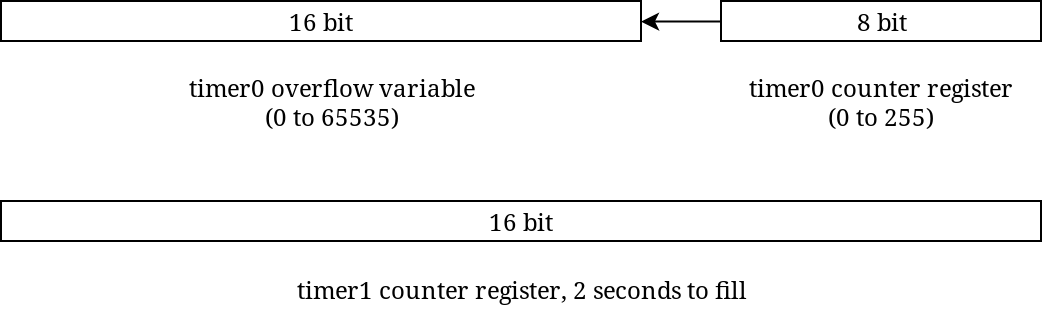
\includegraphics[width=0.7\linewidth]{images/timers}
	\label{fig:timers}
\end{figure}

After the predefined period (2 seconds) has passed, the value of the overflow variable is printed on the LCD screen. The clock frequency can be calculated using these formulas:

$$ f_{clk,exec} = \frac{t0\_overflows \cdot 2^8}{2}\, \left[{\frac{ticks}{seconds} = Hz}\right]$$
$$ f_{clk,sys} = 4 \cdot f_{clk,exec}\,\left[Hz\right] $$

The testing routine has been executed on the board; after a (short) startup stabilization time, the display shows a value equal to:
$$ t0\_overflows = 48825 $$
Which leads to $f_{clk,exec} = 6.2496\,MHz$ and $f_{clk,sys} = 24.9984\,Mhz \approx 25\,Mhz$.\\

A couple of final considerations on this method:

\begin{itemize}
	\item With the current registers configuration, the system clock measurement range is from $512\,Hz$ to $33.55\,MHz$. Precedent experiments had been performed to make sure that the clock frequency was inside this range (it can be set up to $41.667\,MHz$ on the Olimex board).
	\item Being the number of overflows very high, the measurement uncertainty is quite low; even assuming an uncertainty equal to 50 overflows (12800 ticks!) the relative error is around 0.1\%.
\end{itemize}